\section{Introduction}
Carry Protocol aims at building a next generation game infrastructure. The infrastructure aims to fill the gap between Web2 and Web3 games, at the same time creating a fair game economics for blockchain games to thrive as never before. Briefly, Carry introduces an innovative advertising protocol tailored for the game industry, offering the potential for increased revenue for game developers and players. By replacing traditional advertising platforms, this protocol not only enhances the advertising effectiveness for advertisers but also reduces associated costs. \\

The Carry Protocol innovatively bridges the worlds of games and advertising within the web3 space, offering a unique system for showcasing ads within virtual game environments. These advertising spaces, or "slots," are thoughtfully integrated into games, functioning like digital billboards for interactive promotions. This approach aims to create a better and healthier game advertising economics.\\

Moreover, the protocol incorporates a transparent and equitable auction system to allocate advertising space, where the market value of each slot is determined by real-time demand. This system ensures a fair and open process for all participants.\\

The Carry SDK on the side, will provide powerful infrastructure for both Web2 and Web3 games to easily integrate blockchain features. Furthermore, Carry provides adaptive data analysis module for various kinds of games to achieve strategy optimization and service evolution.


\subsection{Motivation}
In this section, we attempt to summarize the primary challenges of the current game market.
\begin{itemize}[leftmargin=*]
    \item \textbf{Failed Incentives:} The dominance of the play-to-earn dual-token economic model in many web3 games, although initially promising, has demonstrated its limitations. Due to its aggressive and singular incentive structure, it often places developers and players in positions of discordant interests, threatening the game’s longevity \cite{leonardos2020oceanic}. In the later stages of the vast majority of play-to-earn games, due to the singularity of incentive mechanisms, players can solely profit by selling their held NFT assets. Regardless of the developers’ efforts to salvage or enhance the game experience, games remain highly susceptible to entering a "death spiral" within a relatively short timeframe. 
    
    For a sustainable future, web3 games necessitate diversified economic mechanisms that foster collaborative wins among developers, players, and other stakeholders.
    
    \item \textbf{Platform Monopoly:} Developers have grown weary of the "Apple tax", which, as a giant advertisement platform, dominates the web2 advertising system and web2 monetization standards by monopolizing user data assets \cite{hovenkamp2020antitrust}. The web2 advertising ecosystem primarily comprises four key players: advertisers, media, advertising platforms, and users. Advertising platforms, by monopolizing user data assets, shape the advertising monetization landscape. However, the advancement of privacy technology and blockchain technology has provided a mature technological solution for a fairer advertising protocol \cite{stallone2023enhancing}.
 
    Both developers and users have a strong demand for a more equitable and efficient advertising ecosystem. The current dominance of giant advertising platforms has significantly impacted business and innovation efficiency.

    \item \textbf{Inability to Analyze Player Intent:} Despite the transformative potential of web3 in games, many developers operate based on speculative insights about player preferences, leading to games that either wane in popularity or serve primarily for asset arbitrage. The heart of this challenge is the absence of effective tools to analyze user behavior within Web3 games. This oversight hinders developers from truly understanding player intent \cite{abeele2020development}. Notably, games like Crypto Kitties, which introduced users to the creation and trade of in-game NFTs, underscore the vast possibilities but also the need for more nuanced player behavior insights.

    Using the crypto-native game ’Loot’ as a case study, it’s evident that following its significant traction within the NFT community, over 20 development teams have emerged with a focus on Loot. These teams are diligently working on an array of games rooted in the foundational model of Loot. However, a minimal number of these endeavors have shown tangible advancement. To solve these issues, the developers and players need to have more interaction during its lifecycle. Native features in web3, for example, predict the market, provide methods for developers to truly interact with players.
 
    As a slogan in the web3 industry goes, "onchain is the new online." Therefore, a multitude of data dimensions can now be easily captured. We need greater insights into users to enhance the efficiency of advertising and games.
\end{itemize}

\subsection{Related Works \& Projects}
The Carry Protocol operates at the intersection of blockchain technology, gaming, and digital advertising, marking a significant step forward in the evolution of Web3 gaming infrastructures. To contextualize Carry's contributions, it's essential to review existing projects and research that have paved the way for innovations in game finance (GameFi), in-game advertising, and blockchain integration within the gaming industry. This section delves into several key projects and areas of work that share thematic or technical overlap with the aims of Carry Protocol.

\subsubsection{Decentraland and Virtual Real Estate}


\href{https://decentraland.org/}{Decentraland} represents a pioneering effort in creating a decentralized virtual world, where users can buy, sell, and manage virtual real estate \cite{guidi2022social}. It stands as a hallmark example of integrating blockchain technology with digital land ownership, offering a vivid parallel to Carry's slot-based advertising model. In Decentraland, landowners have complete control over their parcels, which can be developed to display content, host games, or serve advertisements, similar to Carry's vision of in-game slots as digital real estate for ads.

\subsubsection{Axie Infinity and Play-to-Earn Model Evolution}

\href{https://axieinfinity.com/}{Axie Infinity} revolutionized the GameFi space by popularizing the play-to-earn (P2E) model, where players earn cryptocurrency rewards for gameplay achievements and trading in-game assets \cite{lai2023quantitative}. While Carry Protocol acknowledges the limitations of the early P2E models, it seeks to refine this concept by creating a more sustainable and equitable economic system for all stakeholders, emphasizing the need for diversified economic mechanisms beyond the dual-token models that Axie initially introduced.

\subsubsection{Brave Browser and Attention-Based Advertising}

The \href{https://brave.com/}{Brave Browser} and its associated Basic Attention Token (BAT) introduce a novel approach to online advertising, where users are rewarded for viewing ads \cite{trotz2019times}. This model aligns closely with Carry's ethos of fair compensation for engagement. Carry extends this philosophy into the gaming domain, proposing a system where players and developers benefit directly from ad integration, suggesting a move towards more interactive and player-focused advertising strategies within the game industry. Moreover, Carry provides a general infrastructure for both traditional and emerging (Web3) games to integrate blockchain features, which is not achieved by the Brave Browser.

\subsubsection{Enjin and Asset Tokenization}

\href{https://enjin.io/}{Enjin} has been a frontrunner in providing an ecosystem for creating, managing, and integrating tokenized digital assets into games and apps. By allowing assets to be tokenized on the blockchain, Enjin facilitates true ownership of in-game items, mirroring Carry's concept of slots as tradeable digital assets \cite{marin2023review}. This parallel underscores the broader trend towards asset tokenization in gaming, enhancing the depth and liquidity of virtual economies.

\subsubsection{The Sandbox and User-Generated Content}

The \href{https://www.sandbox.game/}{Sandbox} is a user-generated content (UGC) and gaming platform that empowers players to create, own, and monetize their gaming experiences on the Ethereum blockchain \cite{truby2020fintech}. It exemplifies the potential of blockchain to democratize content creation within virtual worlds. Carry Protocol's slot-based advertising model can be seen as an extension of this democratization, where advertising spaces become a canvas for creative expression and economic participation by developers and players alike.

\subsubsection{Aavegotchi and DAO Governance in Gaming}

\href{https://aavegotchi.com/}{Aavegotchi} stands out for its integration of decentralized finance (DeFi) principles with non-fungible tokens (NFTs) within a gaming context, governed by a Decentralized Autonomous Organization (DAO) \cite{lin2023survey}. The project highlights the potential for community-driven governance models in shaping game development and economic policies, resonating with Carry's aim to foster collaborative wins among all participants in the gaming ecosystem.

\subsubsection{Comparison Analysis}

In examining these related works and projects, it's clear that the Carry Protocol is not operating in isolation but rather building upon a rich foundation of innovation in blockchain, gaming, and digital advertising. By learning from the successes and limitations of these precedents, Carry aims to forge a new path that addresses the challenges of failed incentives, platform monopolies, and the need for deeper insights into player behavior. As the blockchain and gaming landscapes continue to evolve, projects like Carry Protocol will play a crucial role in shaping the future of digital entertainment, advertising, and community engagement.

\subsection{Contributions}
\subsubsection{Slot-based Advertising Paradigm}
At the heart of the Carry Protocol lies the innovative concept of a "slot," a transformative idea designed to bridge the worlds of advertising and on-chain games. In its essence, a slot is a unique digital real estate where advertisements can be strategically placed, integrated seamlessly into the virtual environments of games or other digital platforms.

\begin{figure}[h]
    \centering
    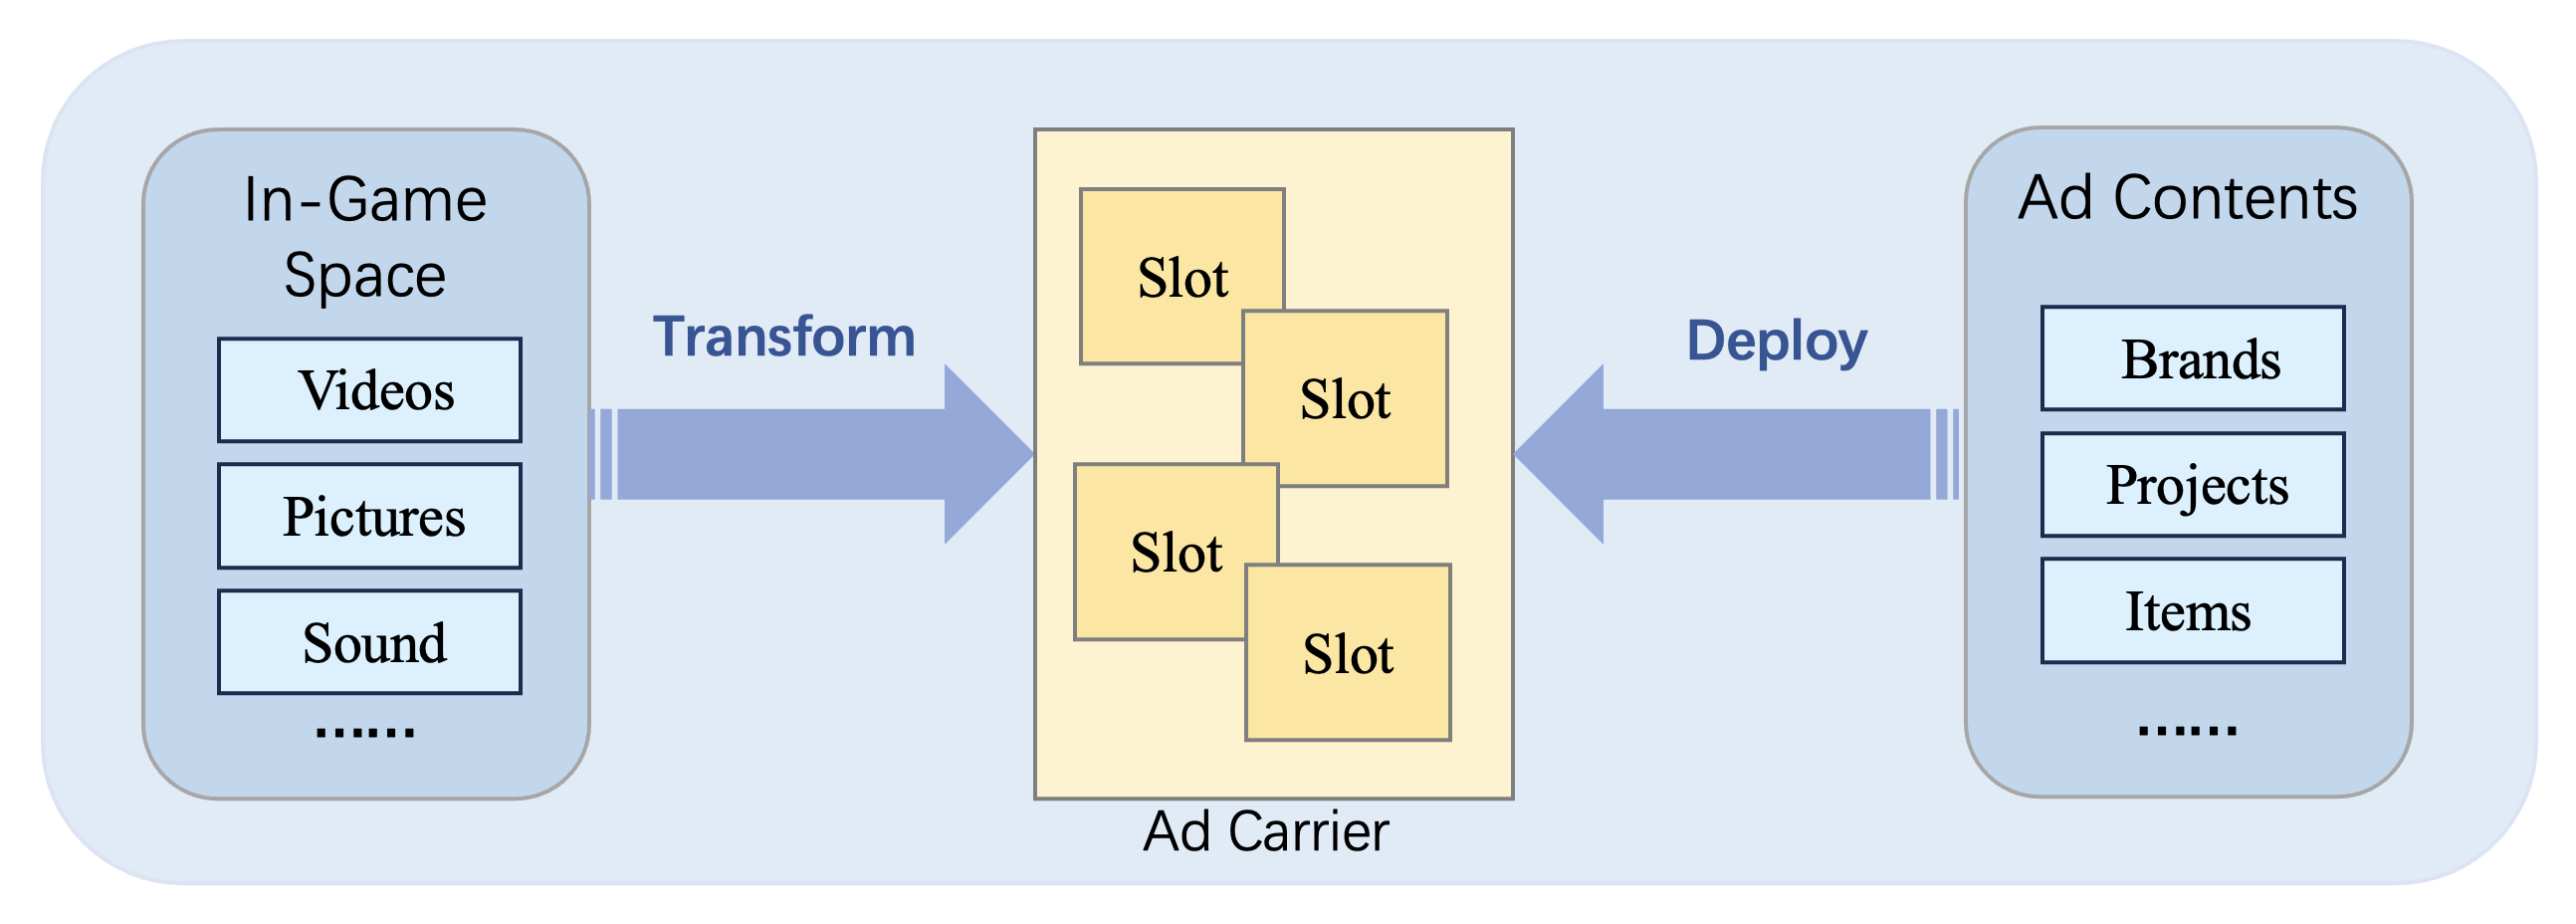
\includegraphics[width=0.7\textwidth]{Slot Design.png}
    \caption{Slot Design}
    \label{fig:slot_basic}
\end{figure}

\begin{itemize}
    \item Every slot is inherently tied to a designated game, taking forms such as visual spaces for graphics, character-specific sound effects, or virtual companions roaming the digital environment.
    \item Beyond their in-game presence, slots hold asset value and can be traded or transferred among participants.
    \item Slots can be a carrier of various types of media, videos, pictures etc.
\end{itemize}

Imagine you're playing an online game, and as you explore, you see ads on billboards or even on items like a character's backpack. These are what we call "slots" in the Carry Protocol. Think of a slot like a piece of virtual real estate where ads can live. These slots are valuable to advertisers and can be bought, sold, or traded just like other virtual items in the game.

% As shown in Figure \ref{fig:billboard}, a billboard in an RPG game is a type of virtual space that can be abstracted as slots.

% \begin{figure}[h]
%     \centering
%     \includegraphics[width=0.7\textwidth]{billboard.jpg}
%     \caption{Example of Advertisement Space in Games: when playing RPG games, the billboard can be abstracted as a slot space where advertisements can be placed on to.}
%     \label{fig:billboard}
% \end{figure}

Slots are versatile. They can show video ads, become part of the game scenery, or even be part of the outfit your character is wearing. They're designed to fit into the game naturally, so they're interesting rather than annoying.

The worth of these ad spaces can go up or down. For example, a slot right where players hang out the most could be worth a lot because more players will see the ad there, while a slot off in a quiet corner might not be as valuable.

The Carry Protocol is all about changing up the game when it comes to ads. These slots are active parts of the game that can change based on how players interact with them and what advertisers want to try. They're a new way to think about ads in games, making sure that players' experiences come first.


\subsubsection{One-Stop Game Infrastructure}

As early blockchain experts and game developers merged, there appeared to be innumerable hours spent learning seemingly nonessential concepts foreign to each other’s native skillsets. Many developers suggested that fortes were being unnecessarily overcomplicated. They needed a tool to realize their function; comprehending its mechanism should be optional education.

Without a proper foundation, an ecosystem cannot thrive. Carry SDK was developed precisely for this purpose; it’s a secure and easy-to-use library of standardized blockchain tools, or rather, a one-stop metaverse infrastructure platform for the game ecosystem. Using Carry SDK, developers no longer need to be intimidated or hindered by the security and complexity of blockchain technology. The entry threshold is lowered, and in terms of cost, eliminated. All interested gamers can expect increased playability as a result.


\subsubsection{Adaptive Game Data Analysis}
The Carry Protocol introduces an Adaptive Data Analysis Module for Web3 gaming, offering real-time insights into in-game advertising effectiveness through Performance Benchmark Metrics. This innovation enables game developers and advertisers to optimize ad placements and content dynamically, ensuring ads enhance rather than detract from the gaming experience.

By leveraging strategy simulation and comprehensive evaluation metrics, the protocol facilitates precise adjustments and targeted experiments with advertising strategies. This approach not only improves monetization strategies for developers but also ensures advertisements are engaging and relevant to the player community, marking a significant advancement in the integration of blockchain technology with the gaming industry.


\subsection{Organization}
The reminder of this Whitepaper are organized as follows. First, we introduce the proposed novel slot-based advertising paradigm, the general launching infrastructure for both Web2 and Web3 games, and the adaptive data analysis module in Section 2-4, respectively. Second, we demonstrate the designed economics and incentives for various system participants in Section 5. Third, we describe the contract-based protocol implementation and some cryptography-facilitated mechanisms in Section 6. Finally, we conclude this work in Section 7.